\subsection{Operating System}

Most of the \glspl{cpe} run on the 32-bit \gls{mips} version of the Linux Kernel. The identification process was made by either executing commands on the device’s shell, as shown in Figure \ref{figure:checking_cpe_operating_system}, or by inspecting the firmware image installed. Unfortunately, not all devices had their operating system identified, they most likely don’t run Linux. 

\begin{figure}[h]
    \centering
    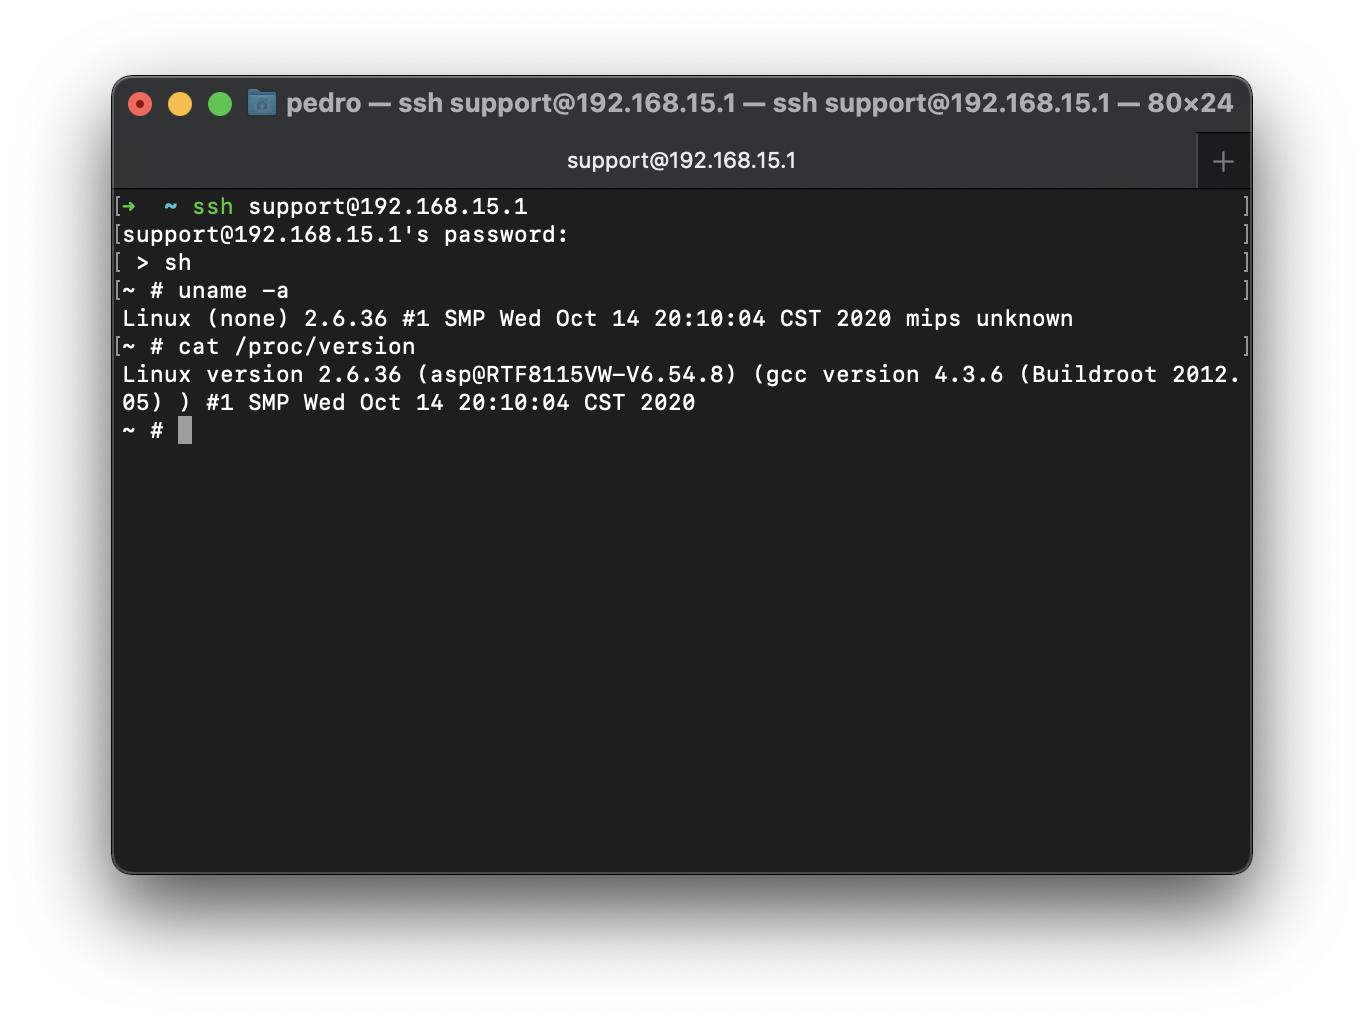
\includegraphics[width=\linewidth]{contents/cpes-and-research-data/operating-system/checking-cpe-operating-system.png}
    \caption{Checking \gls{cpe} Operating System}
    \label{figure:checking_cpe_operating_system}
\end{figure}

Table \ref{table:cpes_oses} presents the operating system identified on each \gls{cpe}.

\begin{table}[h]
    \makebox[\linewidth]{
        \begin{tabular}{c|>{\centering\arraybackslash}m{\linewidth}}
            \thead{\gls{cpe} Identifier} & \thead{Operating System} \\
            \hline
            \gls{cpe}-0 & unknown \\
            \gls{cpe}-1 & unknown \\
            \gls{cpe}-2 & unknown \\
            \gls{cpe}-3 & unknown \\
            \gls{cpe}-4 & \texttt{Linux version 3.4.11-rt19+ (openwrt@sw3-pc) (gcc version 4.6.2 (Buildroot 2011.11) ) \#1 SMP PREEMPT Thu Jun 18 13:46:11 CST 2020} \\
            \gls{cpe}-5 & \texttt{Linux version 2.6.36 (asp@RTF8115VW-V6.54.8) (gcc version 4.3.6 (Buildroot 2012.05) ) \#1 SMP Wed Oct 14 20:10:04 CST 2020} \\
            \gls{cpe}-6 & \texttt{Linux version 3.4.11-rt19 (andy@iBuild) (gcc version 4.6.2 (Buildroot 2011.11) ) \#1 SMP PREEMPT Mon Dec 11 17:11:19 CST 2017} \\
            \gls{cpe}-7 & \texttt{Linux version 2.6.36 (john@iBuild) (gcc version 4.3.6 (Buildroot 2012.05) ) \#2 SMP Thu Aug 16 19:00:39 CST 2018} \\
        \end{tabular}
    }
    \caption{Operating Systems of the \gls{cpe}s}
    \label{table:cpes_oses}
\end{table}

\FloatBarrier
